\documentclass[11pt,letterpaper,spanish]{article}

\usepackage{amsmath,amsthm,amssymb,amsfonts,amsxtra,amstext,anysize,graphicx}

%% Para los usuarios de windows descomentar esta linea y utilizar acentos normalmente.
\usepackage[utf8]{inputenc}
\usepackage[spanish]{babel}
\usepackage{mathrsfs}
\usepackage{fullpage}
\usepackage{verbatim}
\usepackage{graphicx}
\usepackage{subfigure}
\usepackage{wrapfig}
\usepackage{esint}
\usepackage{epsfig}
\usepackage{epstopdf}
\usepackage{multirow}
\usepackage{caption}
\usepackage{hyperref}
\usepackage{float}
\usepackage{color}
\usepackage{longtable} 
\usepackage{pdfpages}% Se utiliza para poder
%\newcommand{\parrafo}[1]{\paragraph{#1}\mbox{}\\}


%% LaTeX will automatically break titles if they run longer than
%% one line. However, you may use \\ to force a line break if
%% you desire.
\usepackage{color}
\definecolor{gray97}{gray}{.97}
\definecolor{gray75}{gray}{.75}
\definecolor{gray45}{gray}{.45}
\usepackage{listings}
\lstset{ frame=Ltb,
framerule=0pt,
aboveskip=0.5cm,
framextopmargin=3pt,
framexbottommargin=3pt,
framexleftmargin=0.4cm,
framesep=0pt,
rulesep=.4pt,
backgroundcolor=\color{gray97},
rulesepcolor=\color{black},
%
stringstyle=\ttfamily,
showstringspaces = false,
basicstyle=\small\ttfamily,
commentstyle=\color{gray45},
keywordstyle=\bfseries ,
%
numbers= none,
numbersep=15pt,
numberstyle=\tiny ,
numberfirstline = false,
breaklines=true,
}

% minimizar fragmentado de listados
\lstnewenvironment{listing}[1][]
{\lstset{#1}\pagebreak[0]}{\pagebreak[0]}

\lstdefinestyle{consola}
{
basicstyle=\scriptsize\bf\ttfamily,
backgroundcolor=\color{gray75},
}

\lstdefinestyle{C}
{language=C,
}

\begin{document} %%Comienza el documento 
\renewcommand{\tablename}{Tabla}

  
\epsfig{file= figuras/logonitido, width= 2.3 cm} %% Agrega una imagen
    \begin{tabular}{l}%% tabular va con una "l" no con un uno
    Pontificia Universidad Cat\'olica de Chile\\
    Escuela de Ingenier\'ia\\
    Departamento de Ingenier\'ia El\'ectrica\\
  \vspace{1.9 cm}\mbox{}
    \end{tabular}
    \bigskip
 
\begin{center}
\huge{Diseño de pruebas para el integrado ASCI The Bean v2}\\
%\Large{\textbf{}}\\
%\normalsize{3- Sesiones}
\vspace{0.6 cm}
\end{center}
\vspace{0.3 cm}

\section{Introducción}
\par 
El \textit{ASCI The bean V2} implementa la segunda iteración de un \textit{front-end} para un detector destinado a física de partículas. La figura \ref{front-end} presenta un esquema general de este tipo de implementaciones.\\



\begin{figure}[h!]
% XCircuit output "C:/Users/lenovo/Documents/circuitos/frontend.eps.tex" for LaTeX input from C:/Users/lenovo/Documents/circuitos/frontend.eps.ps
\def\putbox#1#2#3{\makebox[0in][l]{\makebox[#1][l]{}\raisebox{\baselineskip}[0in][0in]{\raisebox{#2}[0in][0in]{#3}}}}
\def\rightbox#1{\makebox[0in][r]{#1}}
\def\centbox#1{\makebox[0in]{#1}}
\def\topbox#1{\raisebox{-\baselineskip}[0in][0in]{#1}}
\def\midbox#1{\raisebox{-0.5\baselineskip}[0in][0in]{#1}}
\begin{flushleft}
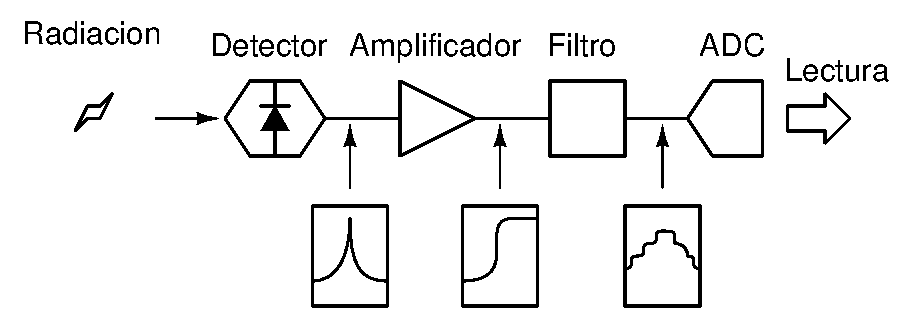
\epsfig{file=C:/Users/lenovo/Documents/circuitos/frontend.eps}\\
% translate x=848 y=672 scale 0.38
\putbox{0.06in}{1.72in}{Radiación}%
\putbox{1.22in}{1.72in}{Detector}%
\putbox{2.22in}{1.72in}{Amplificador}%
\putbox{3.56in}{1.72in}{Filtro}%
\putbox{4.47in}{1.72in}{ADC}%
\putbox{5.14in}{1.72in}{Lectura}%
\end{flushleft}
\caption{\label{front-end} Diagrama general para de un \textit{front-end} de un detector para física de partículas.}
\end{figure}




	
	


A grandes rasgos estos cuentan con tres etapas: un circuito amplificador de carga, encargado de convertir la señal de carga proveniente del detector en una señal de voltaje, posteriormente un filtro también denominado generador de forma de pulsos o \textit{pulse shaper}, el cual se utiliza para reducir la cantidad de ruido en la adquisición tratando habitualmente de maximizar la SNR a la salida del \textit{fornt-end}. Finalmente poseen un bloque encargado de adquirir la información el cual se puede implementar de distintas formas, una de ellas es contar con un conversor análogo digital o ADC que se encargue de adquirir las señales a la salida del \textit{fornt-end} y la convierta en un valor digital para ser leído por alguna electrónica externa habitualmente implementada en una FPGA.


\subsection{Requerimientos}
Debido al contexto en que se encuentra inmerso este trabajo, existen ciertos requerimientos generales heredados que se quieren corroborar de forma extra a los de la implementación realizada. Estos requerimientos se resumen en la tabla \ref{requerimientos}. 
Uno de los aspectos importantes a considerar es que el integrado cuenta con dos modos de operación, el modo estándar de toma de datos (o SDT por sus siglas en ingles) y un segundo modo para propósitos de calibración denominado DCal.




\begin{table}
\centering
\begin{tabular}{|l|l|}
\hline 
Tasa de entrada & 3.25MHz  durante 0.87ms cada 200ms \\ 
\hline 
Modos de operación & Standar data taking(SDT), Detectior Callibration(DCal) \\ 
\hline
Señal de entrada & Hasta 40pC en SDT y hasta 0.74pC en DCal\\
\hline 
Capacitancia de entrada & 65pF \\ 
\hline 
Tolerancia de Radiación & 1 Mrad (SiO2) total ionizing dose \\ 
\hline 
Potencia de consumo & 2.19mW \\ 
\hline 
\end{tabular} 
\caption{\label{requerimientos} Resumen de las especificaciones generales para The Bean V2}
\end{table}


\begin{figure}[!t]
\centering
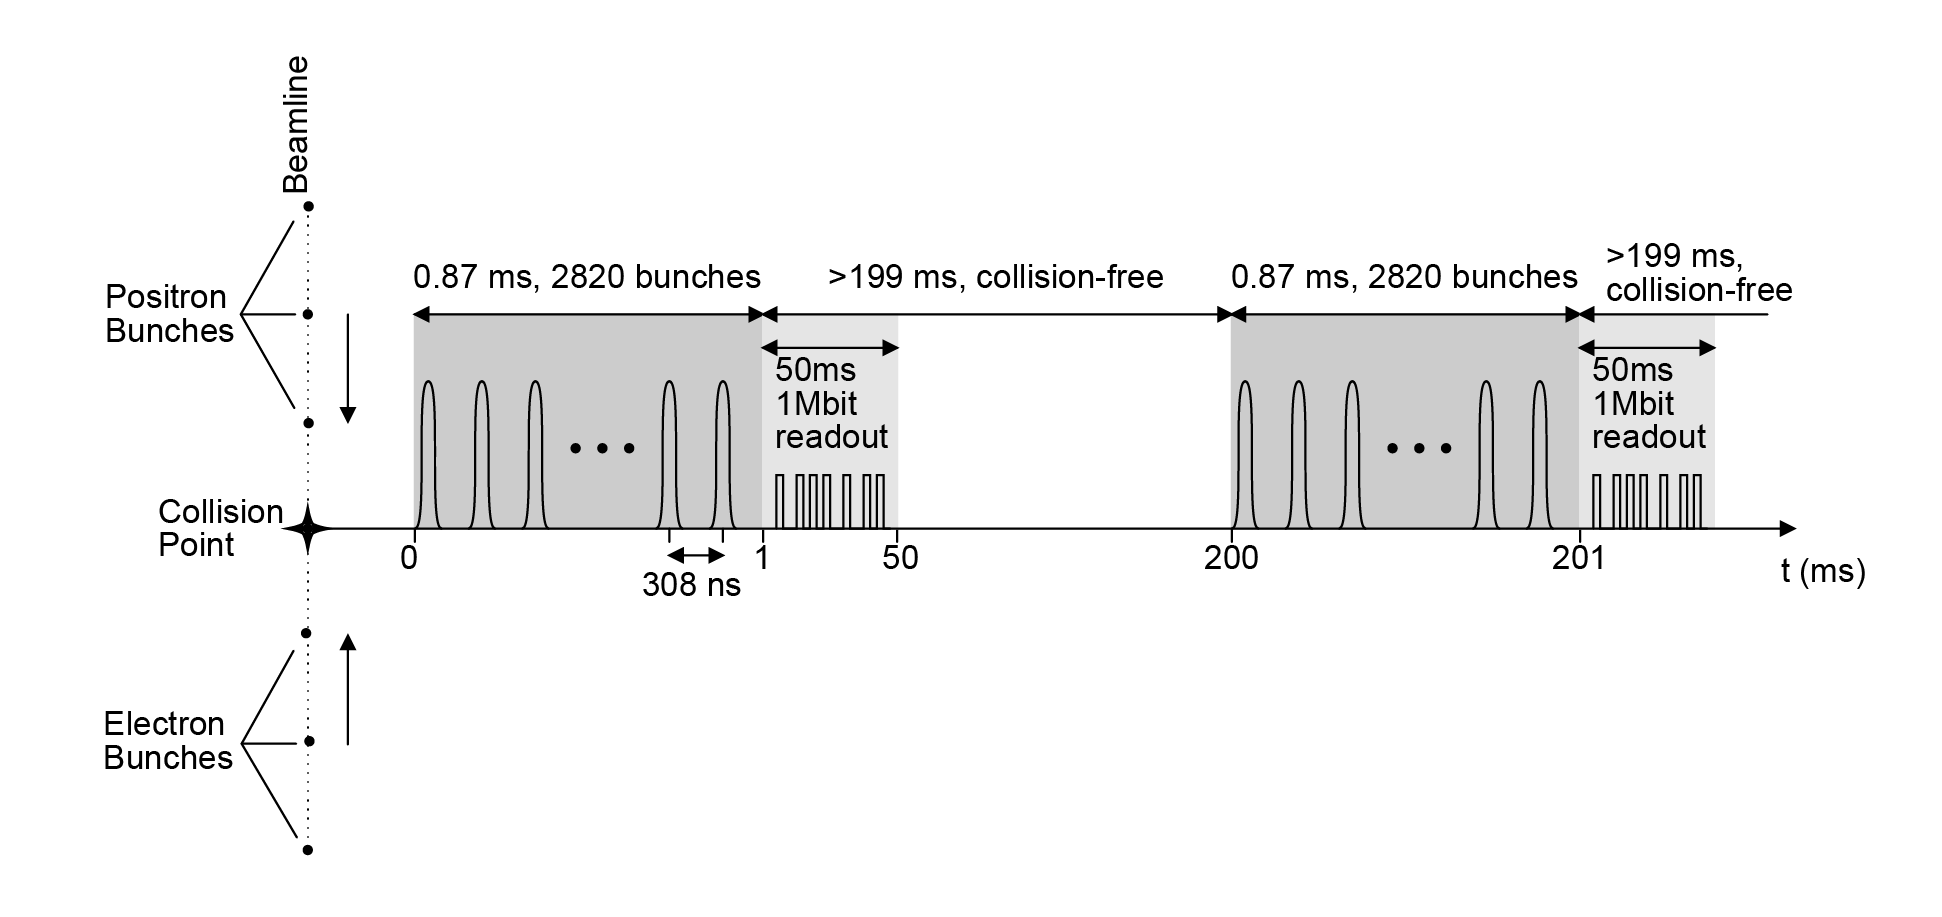
\includegraphics[width=1\textwidth]{./figuras/tiempo.png}
\caption{\label{requisitos de tiempo}Diagrama de tiempo de las colisiones del el tren de pulsos en el colisionador.}
\end{figure}


\section{The Bean V2}
El circuito integrado a probar implementa el esquema mostrado en la figura \ref{front-end} por medio de un amplificador CSA seguido de un filtro generador de formas de pulso que consiste en un integrador  de condensadores conmutados con ganancia ajustable. La figura \ref{layout} muestra el \textit{layout} del integrado diseñado y la tabla \ref{pinout} muestra el \textit{pinout} del empaquetado del chip. 

	
\begin{figure}[!t]
	\centering
	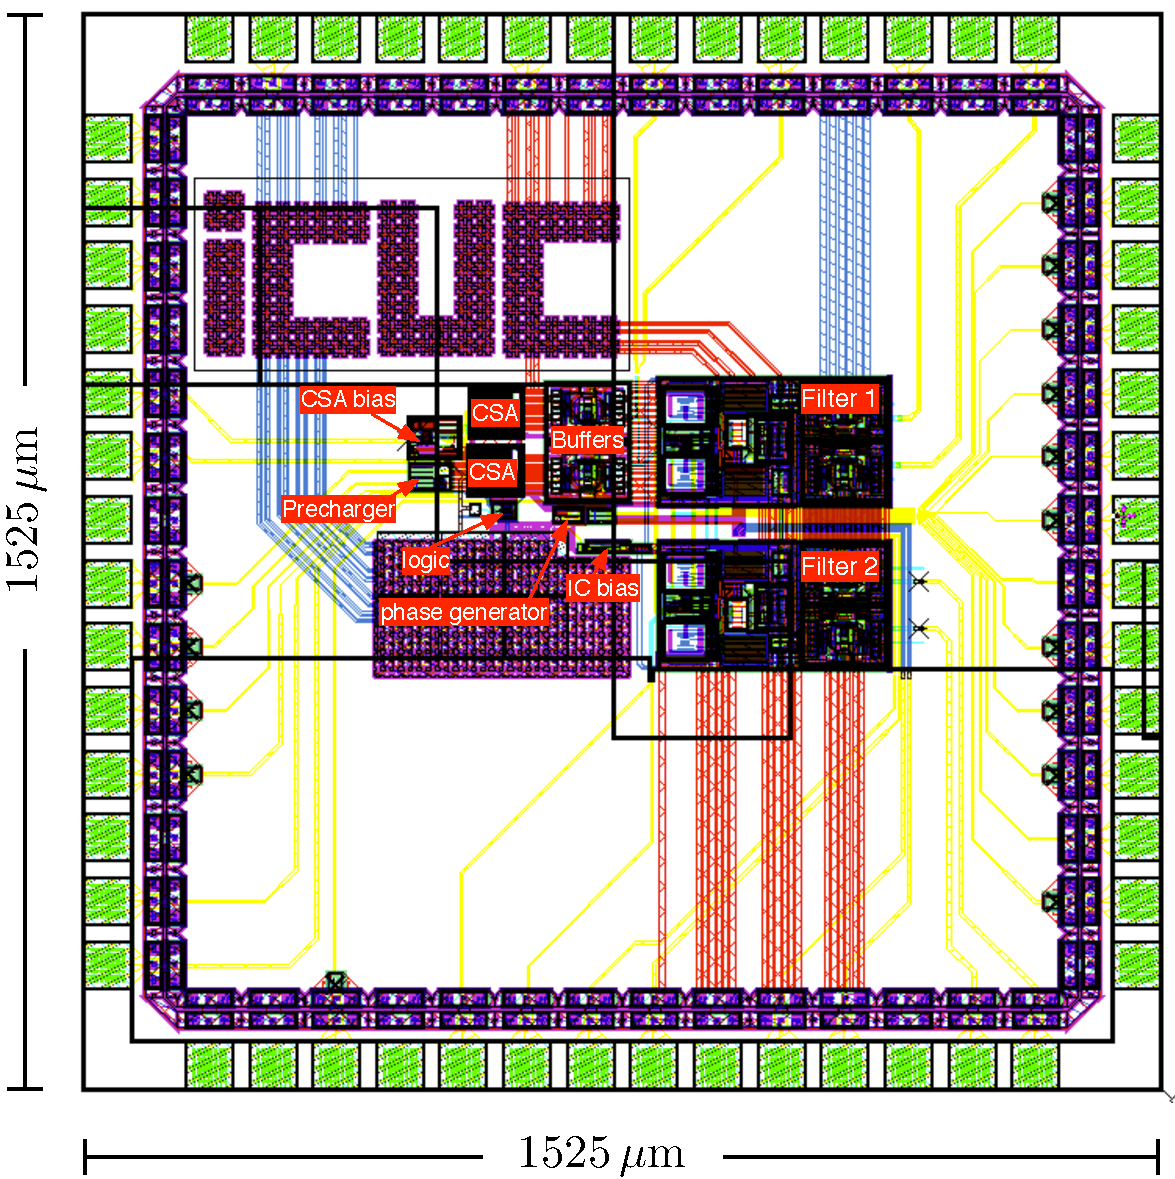
\includegraphics[width=0.7\textwidth]{./figuras/IC_layout}
	\caption{\label{layout}The Bean V2 prototype layout.}
\end{figure}

El esquema general del circuito implementado en este chip se entrega en la figura \ref{thebean}. El integrado cuenta con un bloque CSA el cual recibe la señal de entrada, \verb+Vin_csa+, desde el detector y se encarga de generar un escalón de voltaje proporcional a la cantidad de carga inyectada, también cuenta con un bloque de polarización, un bloque que controla la red de \textit{feedback}, permitiendo cambiar la capacitancia dependiendo del modo de operación y reajustar la re-alimentación, por último cuenta con un bloque de pre-carga, el cual se utiliza para inyectar carga en la entrada con el objetivo de mover el baseline del CSA a un punto que optimice el rango de salida. Ademas cuenta con otro bloque CSA idénticamente al anterior, el cual tiene la salida y la entrada conectadas para poder generar y medir el baseline.

\begin{figure}[!t]
	% XCircuit output "tx_ltspice.tex" for LaTeX input from tx_ltspice.eps
\def\putbox#1#2#3#4{\makebox[0in][l]{\makebox[#1][l]{}\raisebox{\baselineskip}[0in][0in]{\raisebox{#2}[0in][0in]{\scalebox{#3}{#4}}}}}
\def\rightbox#1{\makebox[0in][r]{#1}}
\def\centbox#1{\makebox[0in]{#1}}
\def\topbox#1{\raisebox{-0.60\baselineskip}[0in][0in]{#1}}
\def\midbox#1{\raisebox{-0.20\baselineskip}[0in][0in]{#1}}
\begin{center}
\scalebox{0.4}{
   \normalsize
   \parbox{17in}{
   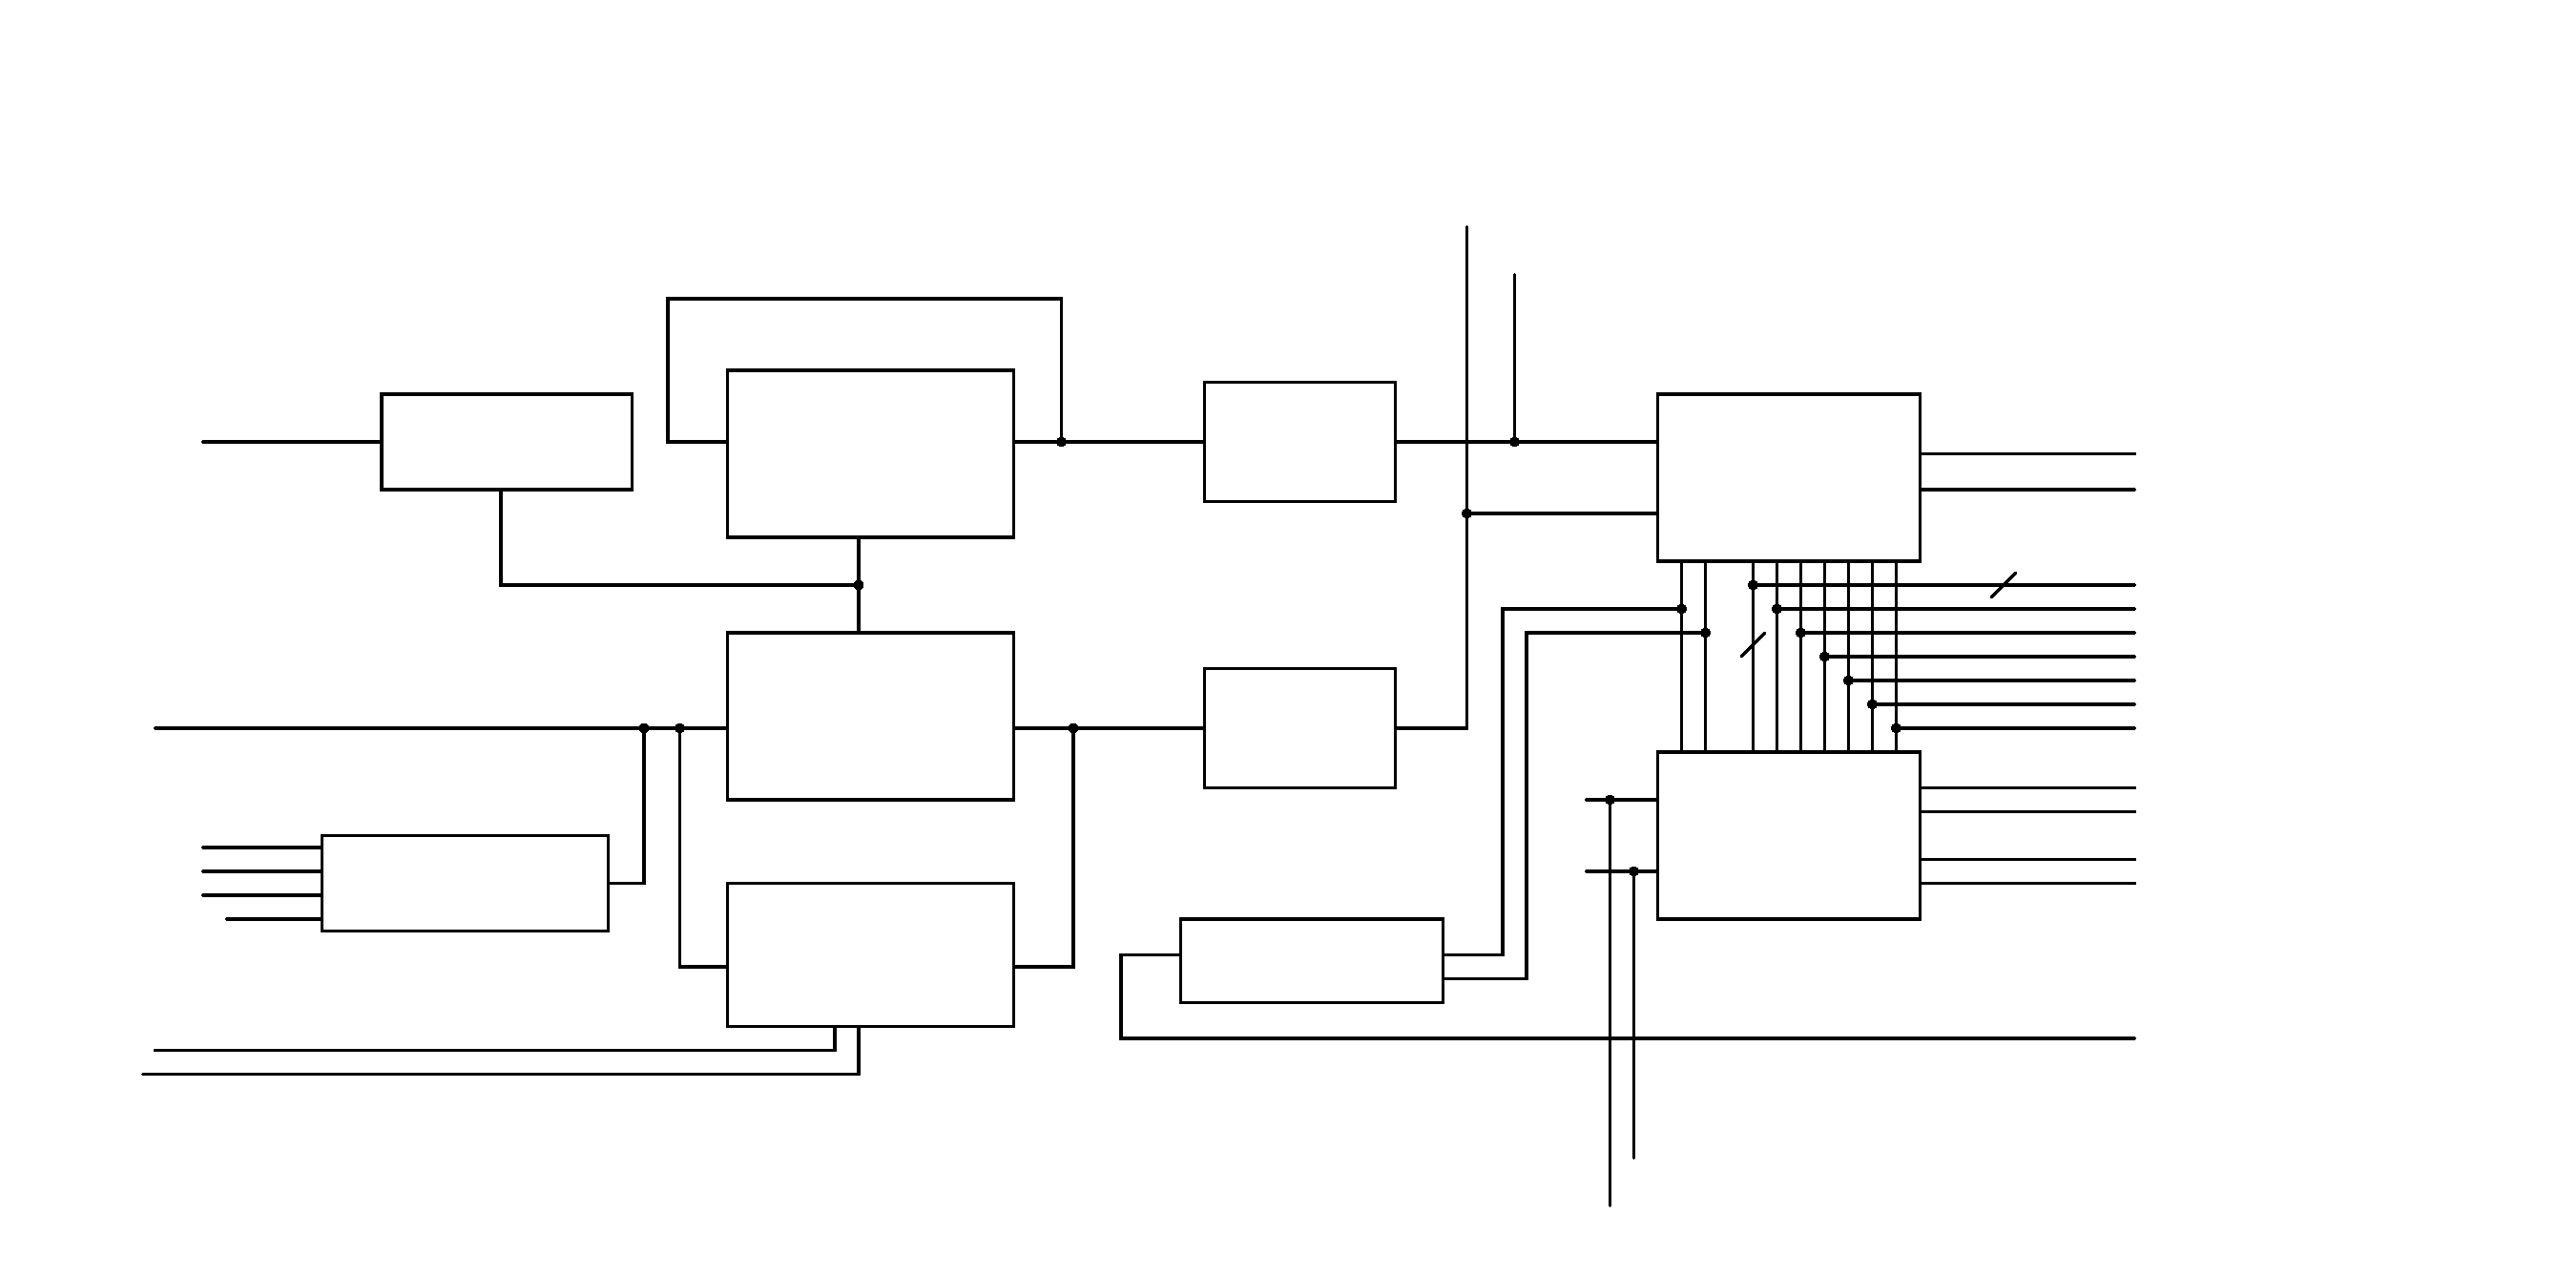
\includegraphics[scale=1]{./figures/theorical/thebeanv2.eps}\\
% translate x=1296 y=1280 scale 0.38
\putbox{0.06in}{5.72in}{1.2}{res\_bias\_ext}%
\putbox{0.06in}{3.72in}{1.2}{Vin\_csa}%
\putbox{0.06in}{2.89in}{1.2}{Vref\_prechar}%
\putbox{0.06in}{2.72in}{1.2}{clk\_prechar1}%
\putbox{0.06in}{2.56in}{1.2}{clk\_prechar2}%
\putbox{0.06in}{2.39in}{1.2}{C\_ext\_prechar}%
\putbox{0.06in}{1.47in}{1.2}{op\_mode}%
\putbox{0.06in}{1.31in}{1.2}{rst\_csa}%
\putbox{2.72in}{5.64in}{1.2}{CSA\_bias}%
\putbox{2.31in}{2.64in}{1.2}{pre\_charger}%
\putbox{5.31in}{2.22in}{1.2}{CSA\_ctrl}%
\putbox{5.31in}{1.89in}{1.2}{feedback}%
\putbox{5.56in}{5.56in}{1.2}{CSA}%
\putbox{5.56in}{3.72in}{1.2}{CSA}%
\putbox{8.56in}{5.64in}{1.2}{buffer}%
\putbox{8.56in}{3.64in}{1.2}{buffer}%
\putbox{8.31in}{2.06in}{1.2}{phase\_gen}%
\putbox{11.97in}{5.39in}{1.2}{Filter}%
\putbox{11.97in}{2.89in}{1.2}{Filter}%
\putbox{14.97in}{4.72in}{1.2}{CS\_Bx}%
\putbox{14.97in}{4.56in}{1.2}{out\_s}%
\putbox{14.97in}{4.39in}{1.2}{Vocm}%
\putbox{14.97in}{4.22in}{1.2}{hold}%
\putbox{14.97in}{4.06in}{1.2}{rst}%
\putbox{14.97in}{3.89in}{1.2}{sgn}%
\putbox{14.97in}{3.72in}{1.2}{Vicm}%
\putbox{14.97in}{5.64in}{1.2}{Vo+\_ch}%
\putbox{14.97in}{5.39in}{1.2}{Vo-\_ch}%
\putbox{14.97in}{3.31in}{1.2}{Vo-\_fil}%
\putbox{14.97in}{3.14in}{1.2}{Vo+\_fill}%
\putbox{14.97in}{2.81in}{1.2}{Vo-\_bp\_fill}%
\putbox{14.97in}{2.64in}{1.2}{Vo+\_bp\_fill}%
\putbox{14.97in}{1.56in}{1.2}{clk}%
\putbox{11.31in}{0.39in}{1.2}{Vin-\_fill}%
\putbox{11.14in}{0.06in}{1.2}{Vin+\_fill}%
\putbox{10.14in}{7.39in}{1.2}{Vout\_csa}%
\putbox{10.47in}{7.06in}{1.2}{baseline}%
   } % close 'parbox'
   } % close 'scalebox'
\end{center}

	\caption{\label{thebean}The Bean V2 prototype layout.}
\end{figure}

Ambas salidas tanto la del CSA \verb+vout_csa+ y el \verb+baseline+ pasan posteriormente por respectivos \textit{buffers}. Las salidas de ambos \textit{buffer} están disponibles para ser leídas en los pines del integrado. Posteriormente ambas señales sirven de entrada para el filtro. Este filtro implementa un integrador totalmente diferencial de capacitores conmutados con capacitancia configurable de forma digital por medio de las señales \verb+CS_Bx+. Ademas de 4 señales de control que controlan el \textit{clock} (\verb+clk+), el signo de la entrada del filtro (\verb+sgn+), la posibilidad de evitar el filtro y obtener a la salida una versión de la entrada(\verb+out_s+),y poder mantener la señal a la salida con el fin de facilitar la lectura(\verb+hold+), ademas de las señales de \verb+vicm+ y \verb+vocm+ que permiten fijar los valores de los voltajes de modo común de entrada y de salida respectivamente. 

Por último, existe una segunda version del filtro para propósitos de pruebas y caracterización, el cual cuenta con las entradas conectadas a pines del integrado, y comparte las señales de control y la polarización con el filtro antes mencionado.

\section{Detalle del integrado}
 

\subsection{El CSA}

El objetivo de este bloque es convertir la carga generada por el detector en una señal de voltaje. La figura \ref{csa} muestra en detalle la forma en que es implementado el CSA. El CSA cuenta con dos condensadores de realimentación los cuales permiten configurar el valor de la capacitancia de realimentación $C_F$, por medio de la señal digital \verb+op_mode+. Así $C_F= C_{Cal}$ en el modo DCal y $C_F= C_{Cal}+ C_{Op}$ en el modo SDT. De este modo, es posible implementar distintas ganancias para los diferentes modos de operación. Por otro lado, la señal \verb+rst_csa+ permite implementar la función de \textit{reset} en la red de realimentación.

\begin{figure}[!h]
	\centering
	% XCircuit output "tx_ltspice.tex" for LaTeX input from tx_ltspice.eps
\def\putbox#1#2#3#4{\makebox[0in][l]{\makebox[#1][l]{}\raisebox{\baselineskip}[0in][0in]{\raisebox{#2}[0in][0in]{\scalebox{#3}{#4}}}}}
\def\rightbox#1{\makebox[0in][r]{#1}}
\def\centbox#1{\makebox[0in]{#1}}
\def\topbox#1{\raisebox{-0.60\baselineskip}[0in][0in]{#1}}
\def\midbox#1{\raisebox{-0.20\baselineskip}[0in][0in]{#1}}
\begin{center}
\scalebox{0.4}{
\normalsize
\parbox{9in}{
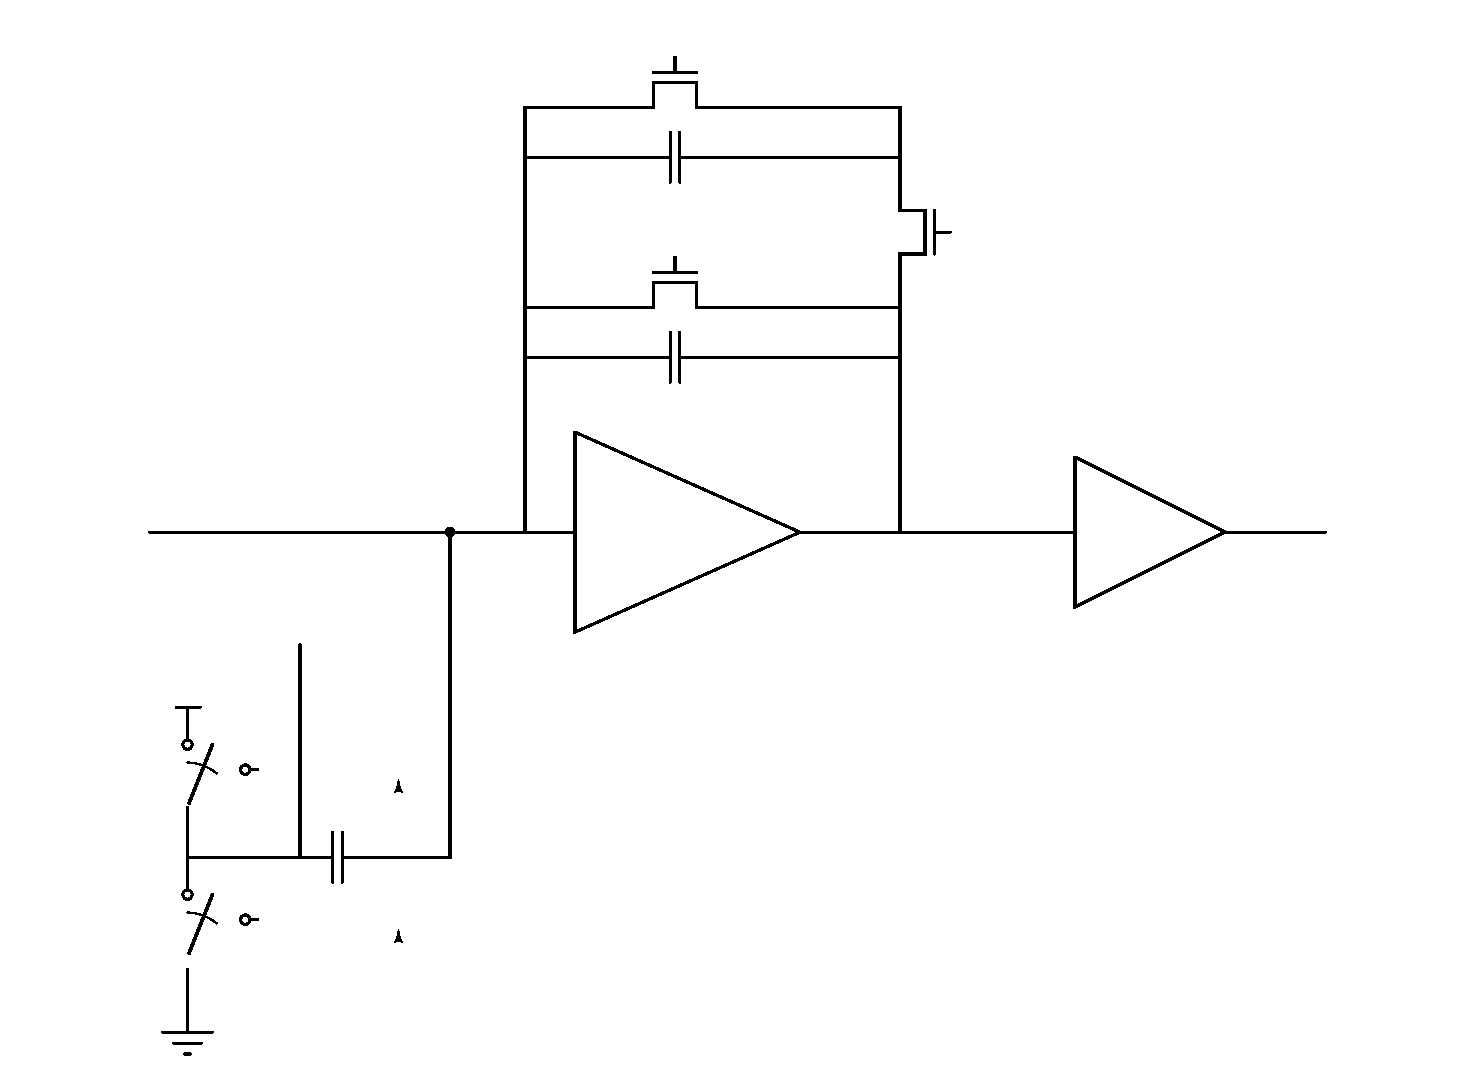
\includegraphics[scale=1]{./figures/theorical/csa_circuit2.eps}\\
% translate x=1152 y=860 scale 0.38
\putbox{0.22in}{3.62in}{1.2}{Vin\_csa}%
\putbox{0.72in}{2.45in}{1.2}{Vref\_pc}%
\putbox{1.56in}{2.87in}{1.2}{Cext\_pc}%
\putbox{4.06in}{5.54in}{1.2}{rst\_csa}%
\putbox{4.14in}{6.79in}{1.2}{rst\_csa}%
\putbox{6.39in}{5.54in}{1.2}{op\_mode}%
\putbox{8.72in}{3.62in}{1.2}{Vout\_csa}%
\putbox{0.14in}{1.87in}{1.2}{$\phi_1$\_pc}%
\putbox{0.06in}{1.04in}{1.2}{$\phi_2$\_pc}%
 } % close 'parbox'
 } % close 'scalebox'
\vspace{-\baselineskip} % this is not necessary, but looks better
\end{center}

	\caption{\label{csa}The Bean V2 prototype layout.}
\end{figure}

 Debido a la configuración con la cual fueron implementados el baseline se establecerá aproximadamente a $V_T$ o $0.5V$, sin embargo la región de operación de alta ganancia se encuentra aproximadamente a los $0.4V$ de los rieles. Para solucionar este problema es que el CSA cuenta con circuito de precarga, el cual inyecta una cantidad conocida de carga para mover el baseline más cerca de los $0.4V$.

\subsubsection{ Pre-charger}
El circuito de precarga fue diseñado para inyectar carga a la entrada del CSA con el objetivo de ajustar el baseline y a la vez para cumplir con propósitos de calibración.
 En la imagen \ref{csa} se muestra una versión simplificada del circuito, el cual esta compuesto de dos switches implementados con transistores y un condensador $C_{PC}$ el cual esta conectado a la entrada del CSA. Para cambiar el valor de la capacitancia de este condensador (modo SDT) existe la posibilidad de conectar un condensador externo en paralelo por medio de la señal \verb+cap_prechar_ext+.
 
 
La forma en que se controla el circuito de precarga se basa en dos señales de clock desfasadas no sobrepuestas. Cuando la primera señal es activa ($\phi_1$), el extremo izquierdo del condensador queda conectado a un voltaje de referencia externo $V_{DD\_ref}$ el cual se puede configurar por medio de la señal \verb+V_ref_prechar+. Posteriormente cuando la segunda señal es activa ($\phi_2$), el extremo izquierdo es conectada a tierra. En cada transision de $\phi_2$ a $\phi_1$ el condensador inyecta una carga de $Q_{CP}=C_{CP} \cdot V_{DD\_ref}$ en la entrada del CSA. Esto provoca una variación de voltaje en la salida de $\Delta V =-C_{CP} \cdot V_{DD\_ref}/C_F$, en donde $C_F$ es la capacitancia de realimentación. La inyección de carga se realiza justo después de que el CSA es habilitado, reduciendo el voltaje de baseline a la salida. 

\begin{figure}
\def\putbox#1#2#3{\makebox[0in][l]{\makebox[#1][l]{}\raisebox{\baselineskip}[0in][0in]{\raisebox{#2}[0in][0in]{#3}}}}
\def\rightbox#1{\makebox[0in][r]{#1}}
\def\centbox#1{\makebox[0in]{#1}}
\def\topbox#1{\raisebox{-\baselineskip}[0in][0in]{#1}}
\def\midbox#1{\raisebox{-0.5\baselineskip}[0in][0in]{#1}}
\begin{flushleft}
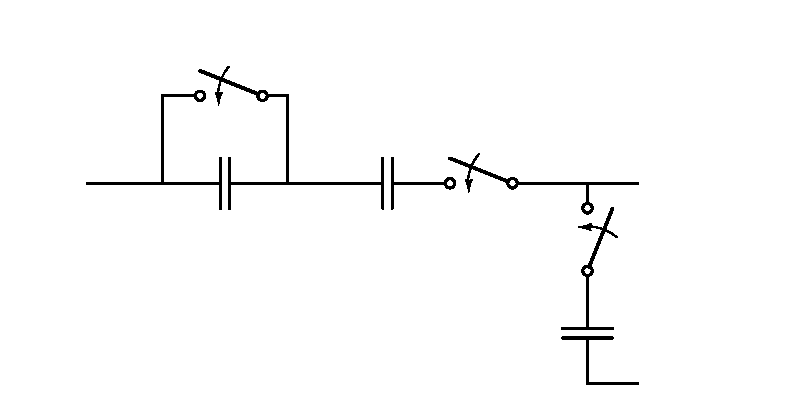
\epsfig{file=./figuras/Injector_de_carga.eps}\\
% translate x=816 y=166 scale 0.38
\putbox{0.06in}{1.42in}{Vin}%
\putbox{1.22in}{2.34in}{JP9}%
\putbox{1.22in}{1.00in}{C36}%
\putbox{1.22in}{0.75in}{0.5pF}%
\putbox{2.31in}{1.00in}{C37}%
\putbox{2.31in}{0.75in}{27pF}%
\putbox{2.81in}{1.75in}{JP10}%
\putbox{4.22in}{1.42in}{Vin\_csa}%
\putbox{4.22in}{0.09in}{Cext\_pc}%
\putbox{3.14in}{0.50in}{C38}%
\putbox{3.14in}{0.25in}{25pF}%
\putbox{3.22in}{1.00in}{JP11}%
\end{flushleft}
\caption{\label{Cir_vin}Circuito de inyección de carga en la tarjeta, para simular un detector.}
\end{figure}

\subsection{Filtro}


\begin{figure}[!h]
	\centering
	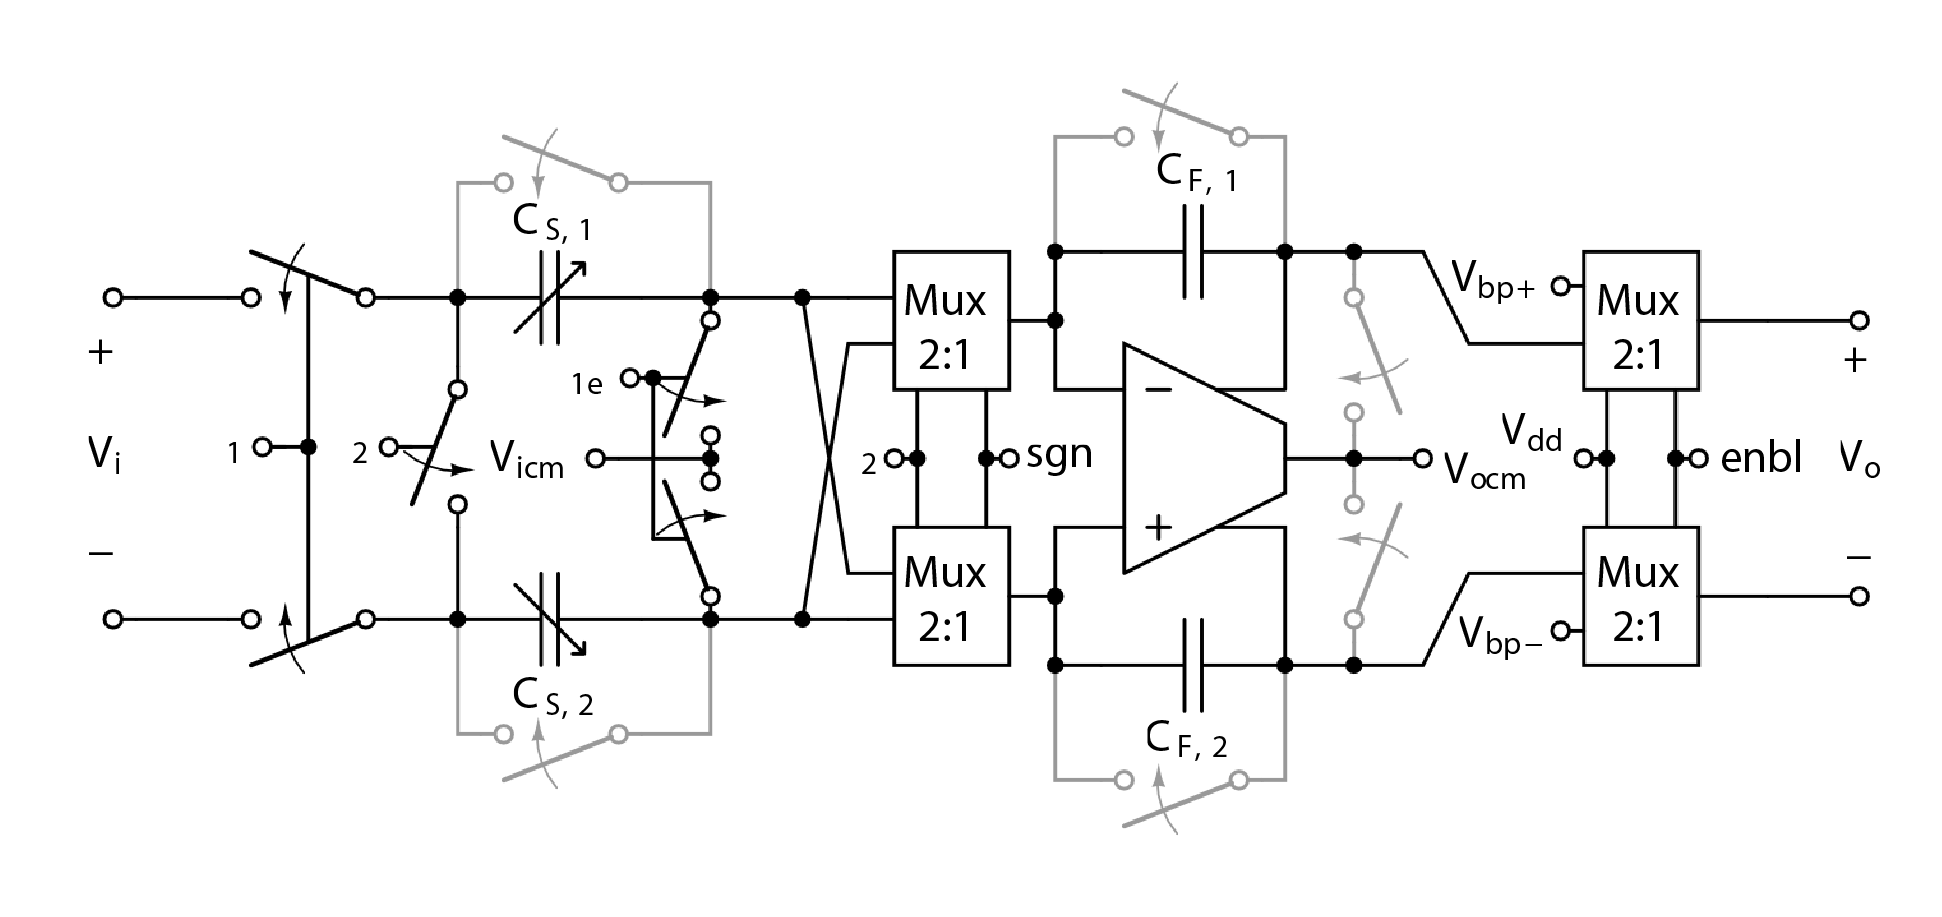
\includegraphics[width=1\textwidth]{./figuras/filtro.png}
	\caption{\label{filtro}The Bean V2 prototype layout.}
\end{figure}

	 

\section{Pruebas y diagramas de tiempo}

\subsection{Diagramas de tiempo}
\begin{figure}[!t]
	\centering
	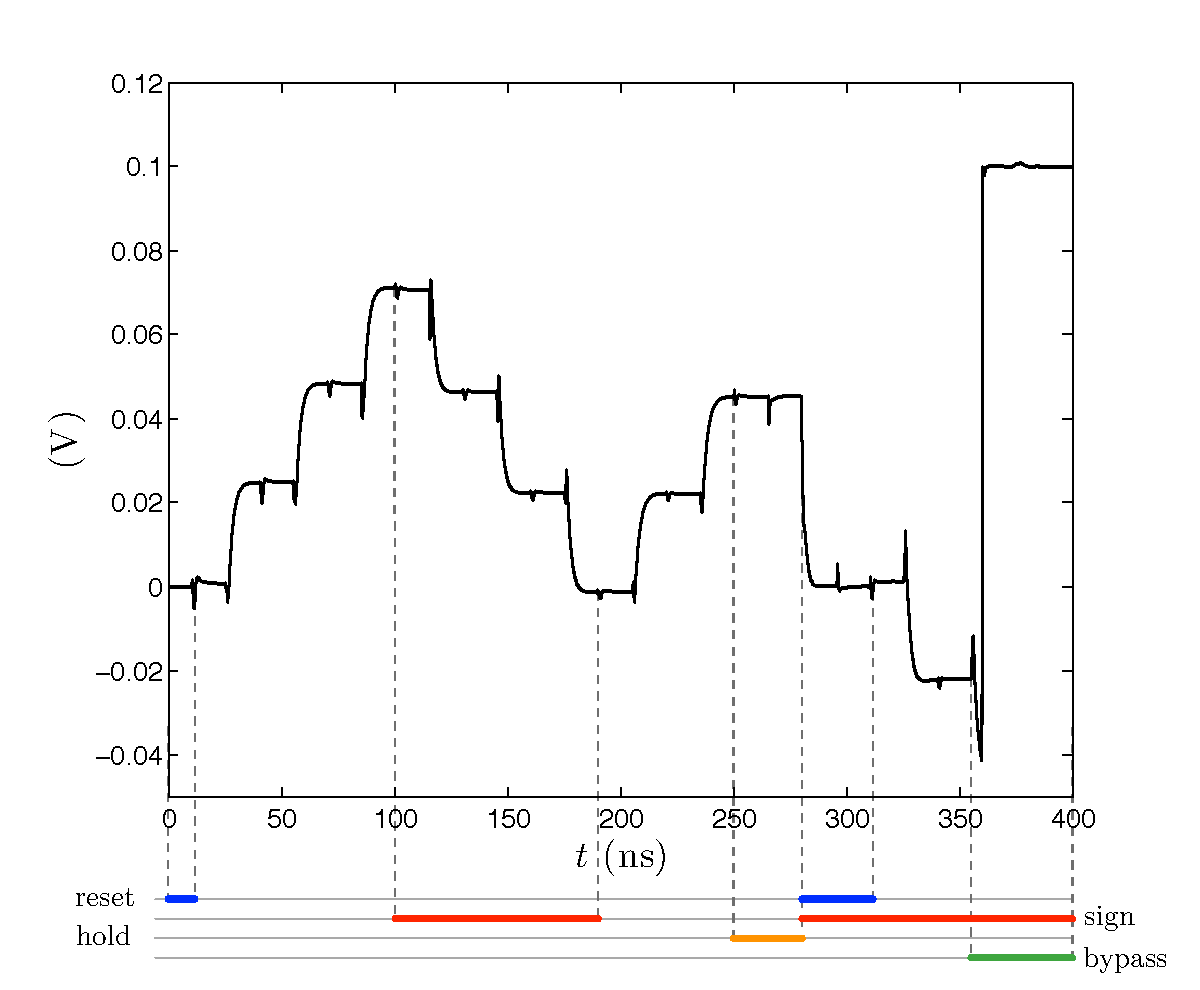
\includegraphics[width=5in]{./figuras/test_filter_after_omni.eps}
	\caption{Filter functionality simulation. $V_\textit{in}=0.1\,V$ and $\text{gain}=0.25\,V/V$.}\label{fig:test_filter_after_omni}
\end{figure}

\begin{figure}[!t]
	\centering
	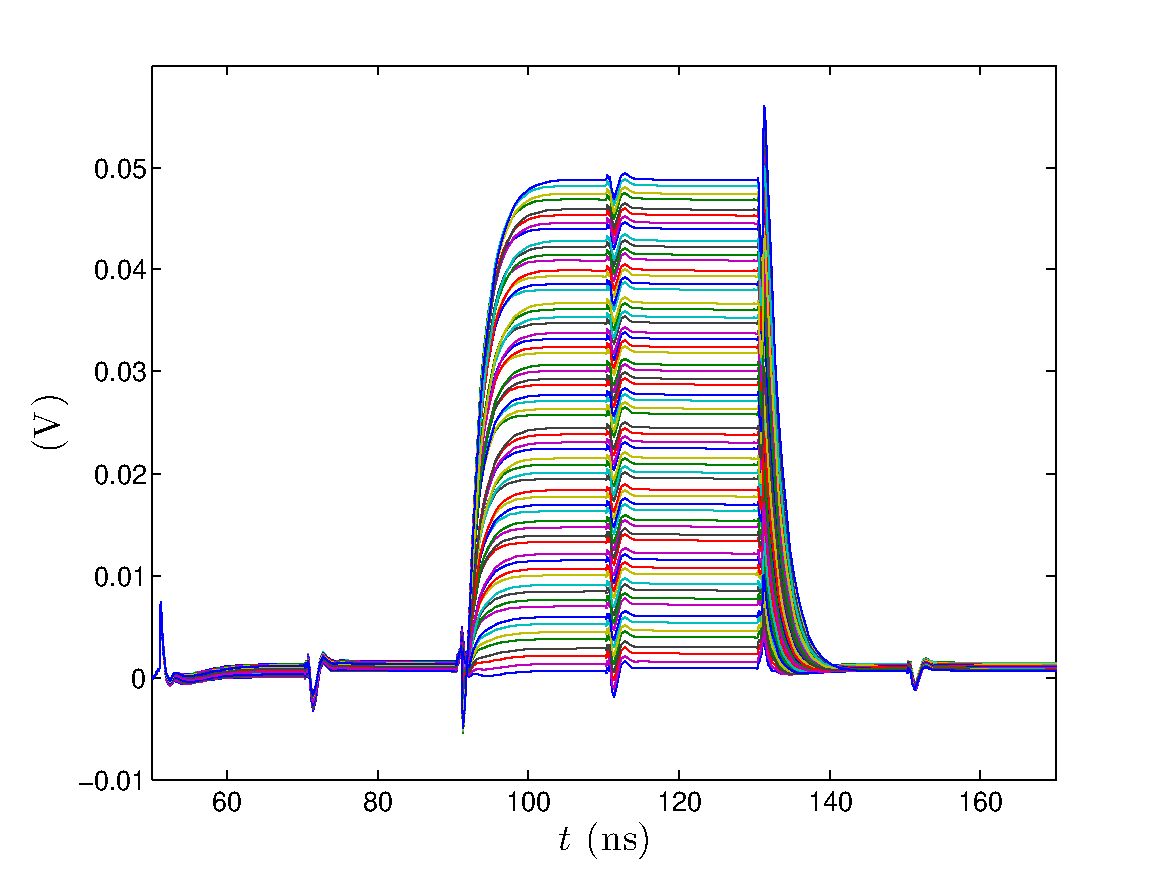
\includegraphics[width=4.4in]{./figuras/gain_curves.pdf}
	\caption[Filter step response for constant input for the 64 possible programmable gains.]{Filter step response for constant input for the 64 possible programmable gains. \mbox{$V_\textit{in}=0.1\,V$} and \mbox{$T_s=40\,\text{ns}$}.}\label{fig:gain_curves}
\end{figure}

\begin{figure}[!t]
	\centering
	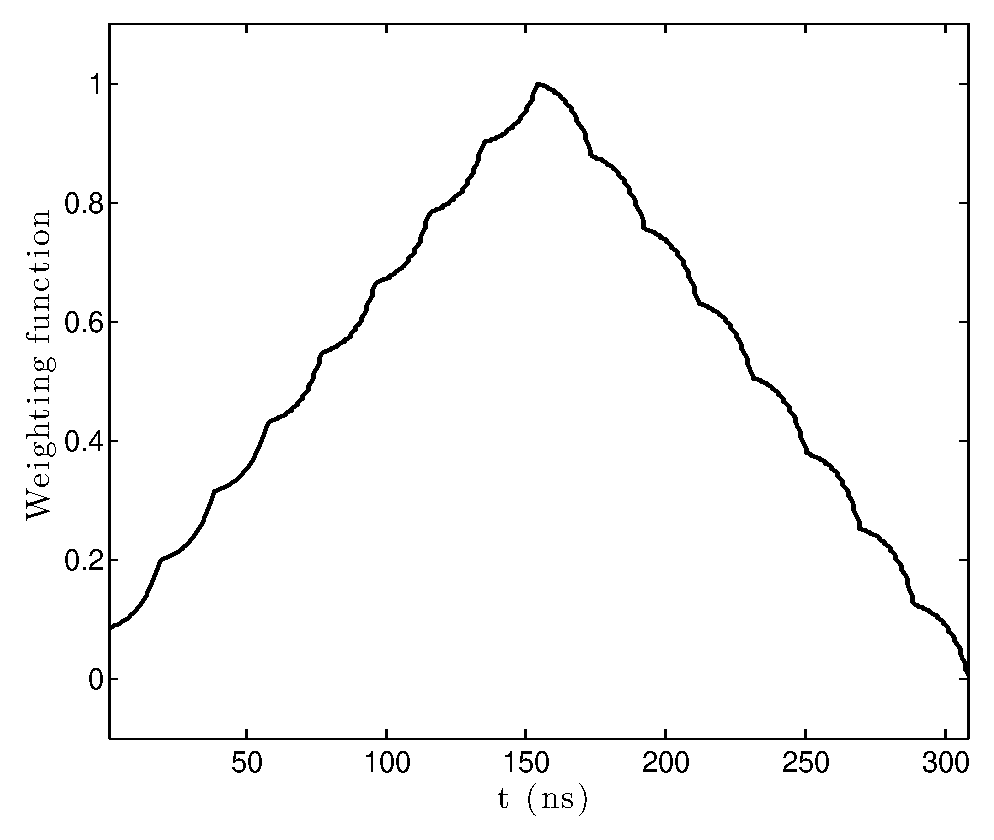
\includegraphics[width=3.6in]{./figuras/sim_wf}
	\caption{SPICE-simulated weighting function. $\tau=8\,\text{ns}$, $N=16$ and $T_s=19.25\,\text{ns}$.}\label{fig:sim_wf}
\end{figure}

\subsection{Diseño de pruebas}

\begin{figure}[!t]
	\centering
	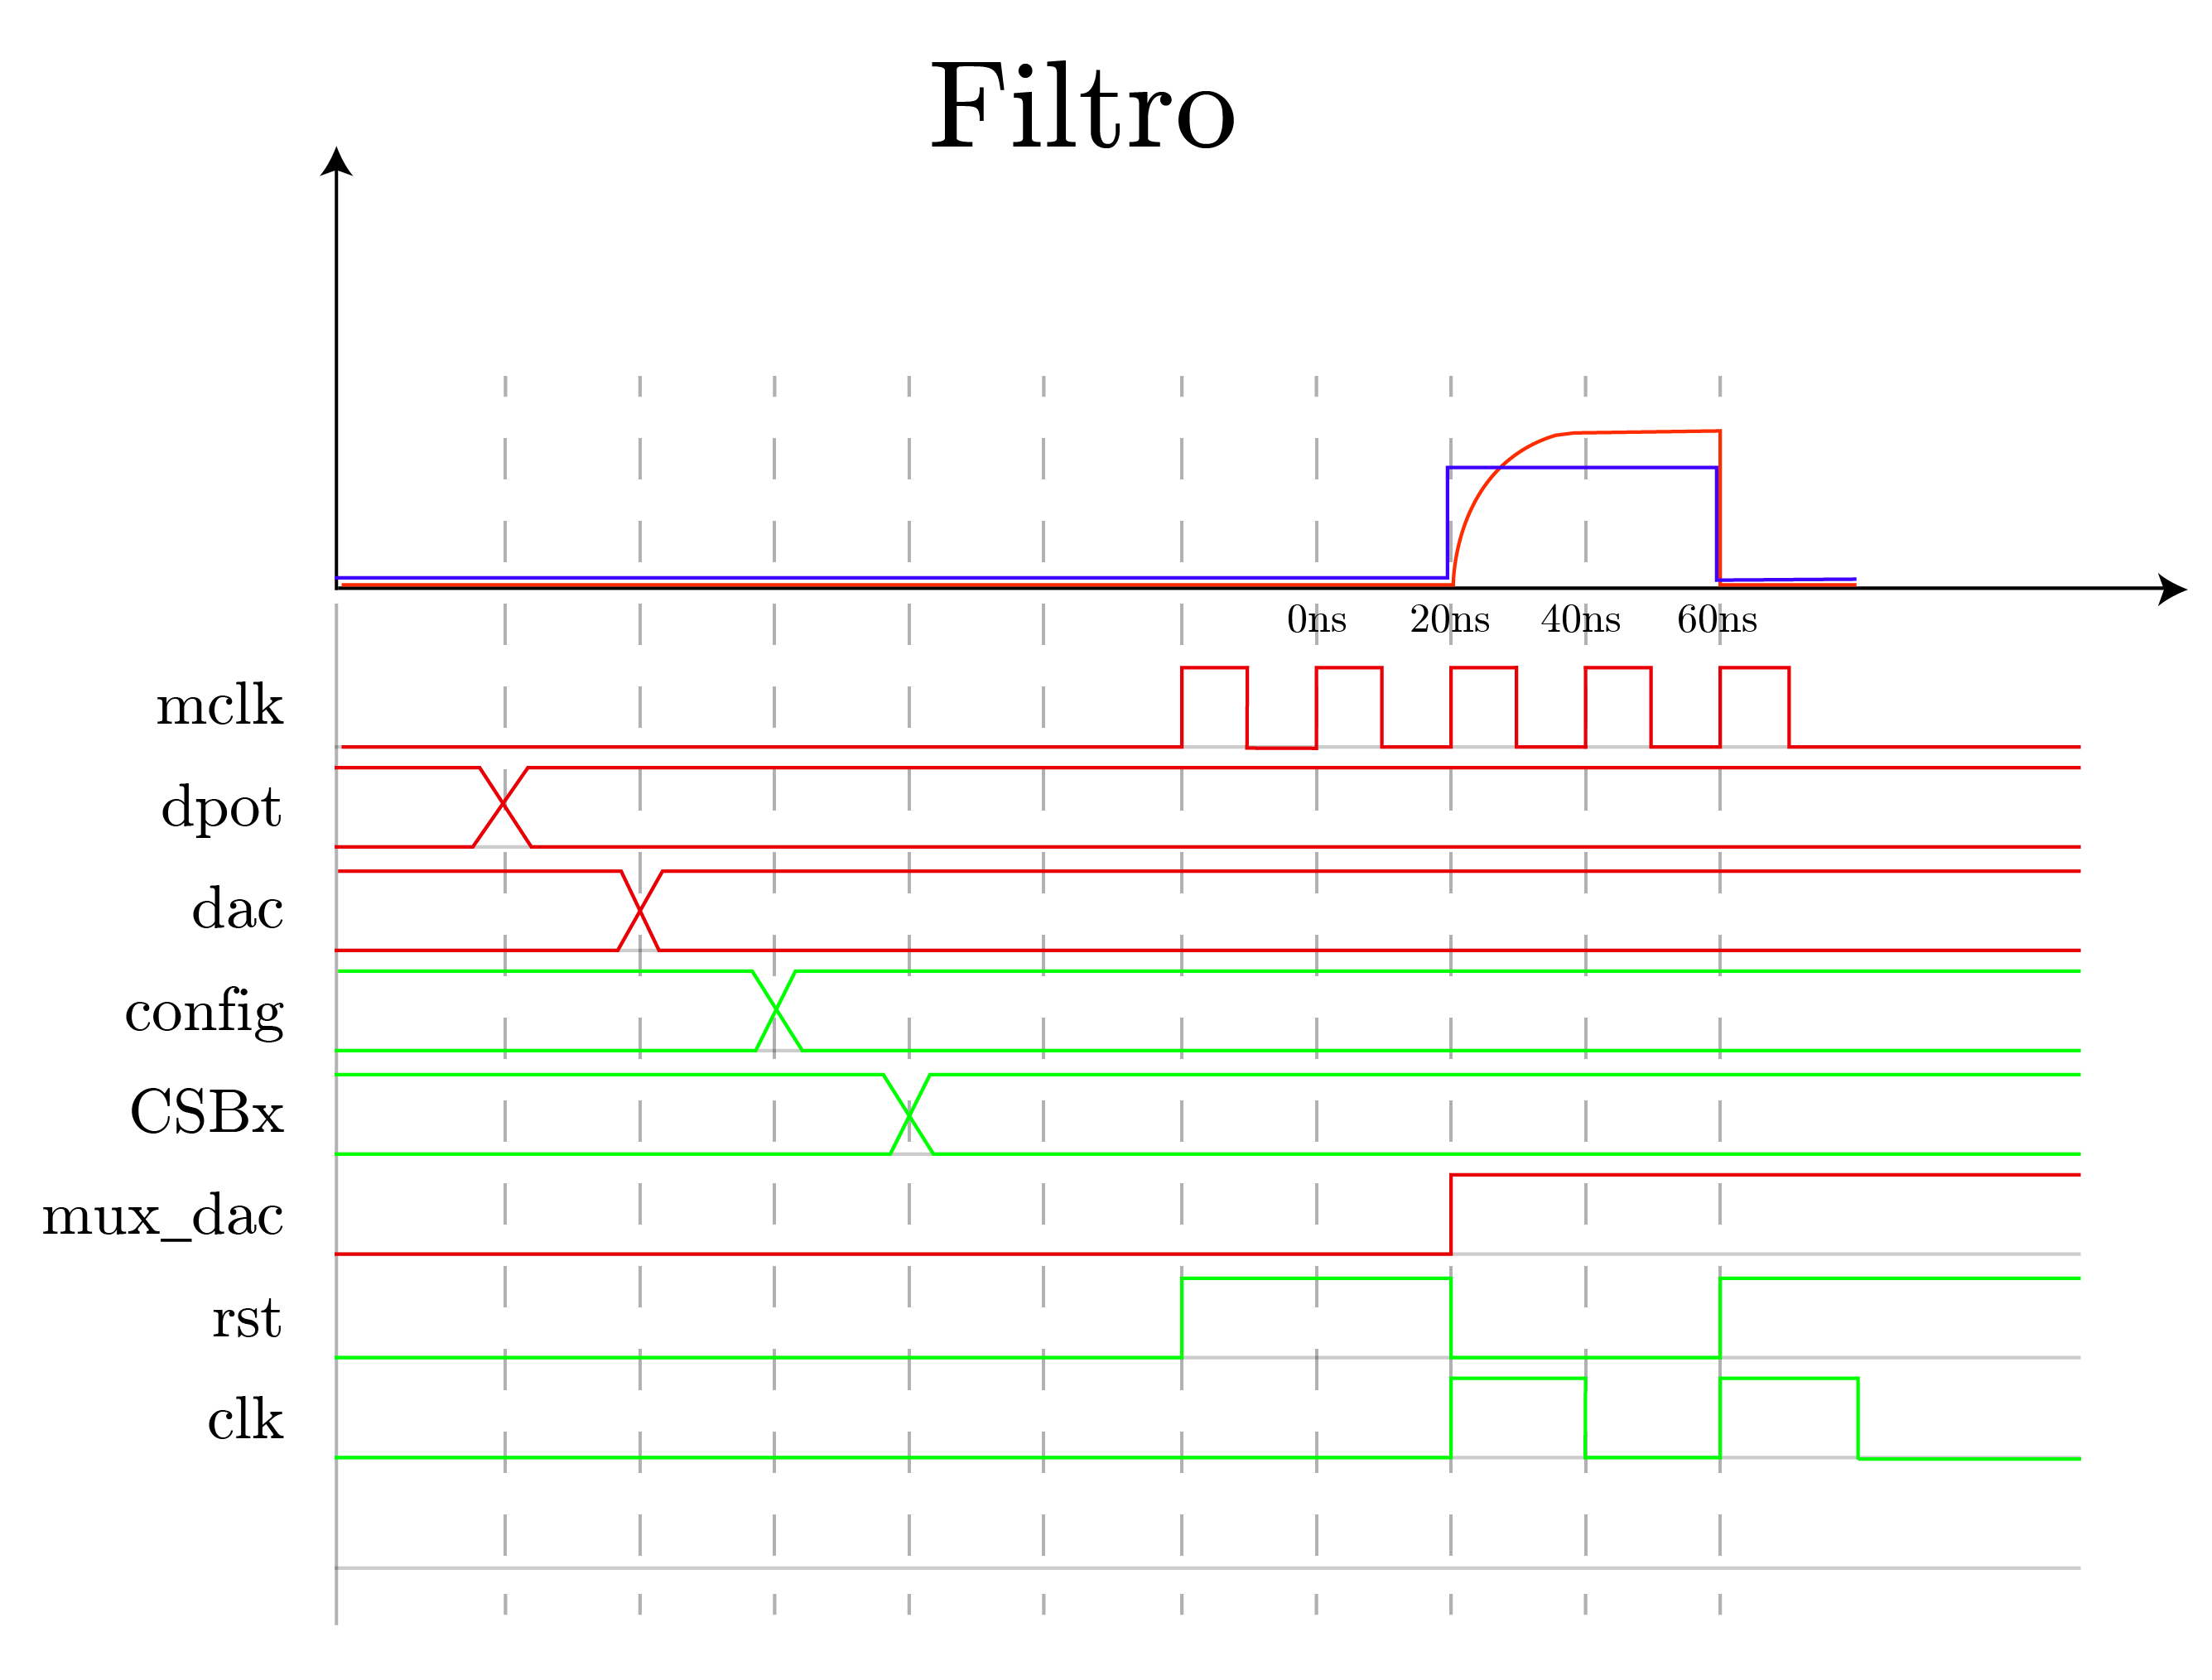
\includegraphics[width=1\textwidth]{./figuras/tiempos_filtro.png}
	\caption{Diagrama de señales para las pruebas realizadas al filtro .}\label{fig:diagramafiltro}
\end{figure}

\begin{figure}[!t]
	\centering
	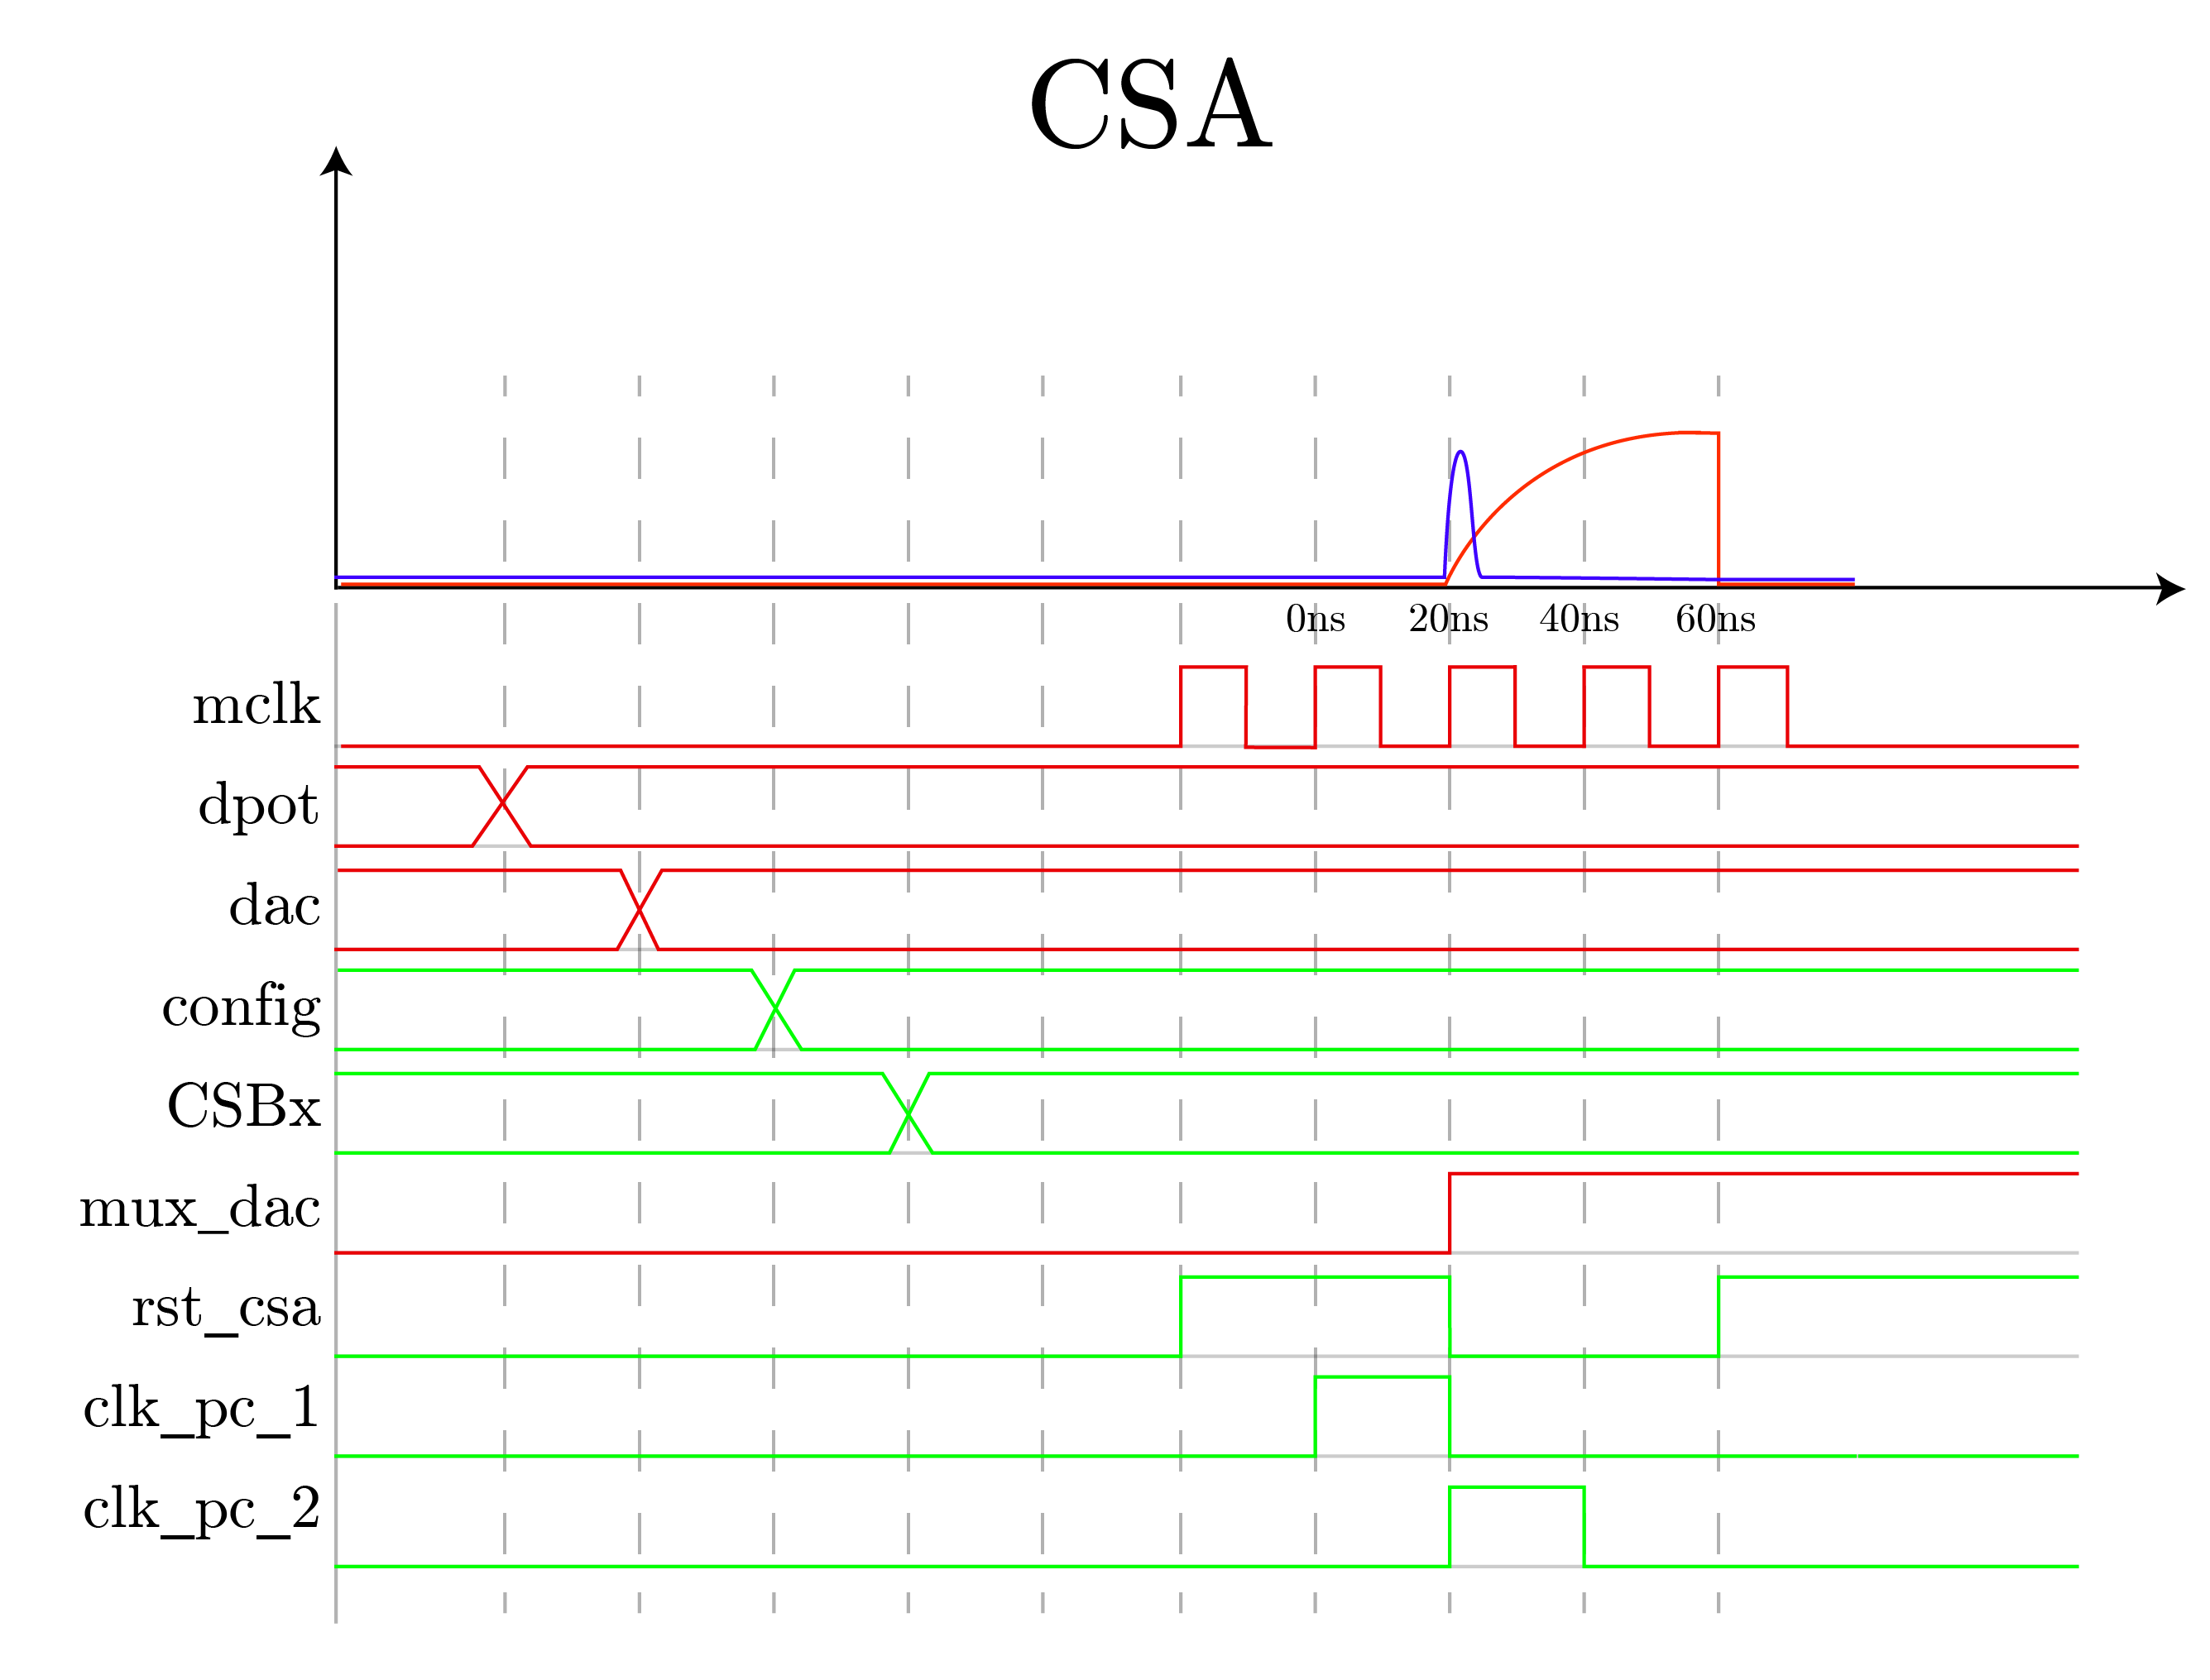
\includegraphics[width=1\textwidth]{./figuras/tiempos_csa.png}
	\caption{Diagrama de señales para las pruebas realizadas al CSA.}\label{fig:diagramacsa}
\end{figure}



\clearpage
\section{Anexo}
El prototipo de The Bean V2 tiene 48 pads y fue bonded a 64-lead package from \mbox{Kyocera} Corporation (KYO). The package KYO part number is QC064307WZ. Table \ref{pinout} shows the Bean V2 pinout.


\begin{center}
\begin{longtable}{|l|l|l|}\hline
{\bf Pin number} & {\bf Pin name} & {\bf Description} \\ \hline\hline
1 & \verb=AGnd= & Analog ground \\\hline
2 & \verb=NC= & No connection \\\hline
3 & \verb=NC= & No connection \\\hline
4 & \verb=NC= & No connection \\\hline
5 & \verb=NC= & No connection \\\hline
6 & \verb=res_bias_ext= & IC bias external resistor \\\hline
7 & \verb=V_ref_prechar= & Reference voltage CSA precharger \\\hline
8 & \verb=NC= & No connection  \\\hline
9 &  \verb=clk_prech1= & CSA precharger clk1  \\\hline
10 & \verb=clk_prech2= & CSA precharger clk2  \\\hline
11 & \verb=op_mode= & Operation mode select \\\hline
12 & \verb=rst_csa= & CSA reset  \\\hline
13 & \verb=NC= & No connection \\\hline
14 & \verb=cap_precharge_ext= & CSA precharger external capacitor \\\hline
15 & \verb=Vin_csa= & Vin CSA \\\hline
16 & \verb=AGnd= & Analog ground \\\hline
17 & \verb=AGnd= & Analog ground \\\hline
18 & \verb=NC= & No connection \\\hline
19 & \verb=NC= & No connection \\\hline
20 & \verb=clk= & IC clock \\\hline
21 & \verb=NC= & No connection \\\hline
22 & \verb=Vi+_fil= & Filter Vi+ \\\hline
23 & \verb=Vi-_fil= & Filter Vi- \\\hline
24 & \verb=Vo+_bp_fil= & Filter bypass Vo+  \\\hline
25 & \verb=Vo-_bp_fil= & Filter bypass Vo- \\\hline
26 & \verb=NC= & No connection \\\hline
27 & \verb=DVdd= & Digital Vdd \\\hline
28 & \verb=DGnd= & Digital Gnd \\\hline
29 & \verb=NC= & No connection \\\hline
30 & \verb=Vo+_fil= & Filter Vo+ (buffered) \\\hline
31 & \verb=Vo-_fil= & Filter Vo- (buffered) \\\hline
32 & \verb=AGnd= & Analog ground \\\hline
33 & \verb=AGnd= & Analog ground \\\hline
34 & \verb=NC= & No connection \\\hline
35 & \verb=out_s= & Filter output selection \\\hline
36 & \verb=Vocm= & Filter Vocm \\\hline
37 & \verb=hold= & Filter hold signal  \\\hline
{\bf Pin number} & {\bf Pin name} & {\bf Description} \\ \hline\hline
38 & \verb=rst= & Filter reset \\\hline
39 & \verb=sgn= & Filter gain sign \\\hline
40 & \verb=Vicm= & Filter Vicm \\\hline
41 & \verb=CS_b0= & Filter CS capacitor bit 0 \\\hline
42 & \verb=CS_b1= & Filter CS capacitor bit 1 \\\hline
43 & \verb=CS_b2= & Filter CS capacitor bit 2 \\\hline
44 & \verb=CS_b3= & Filter CS capacitor bit 3 \\\hline
45 & \verb=CS_b4= & Filter CS capacitor bit 4 \\\hline
46 & \verb=CS_b5= & Filter CS capacitor bit 5 \\\hline
47 & \verb=NC= & No connection \\\hline
48 & \verb=AGnd= & Analog ground \\\hline
49 & \verb=AGnd= & Analog ground \\\hline
50 & \verb=Vo+_ch= & Channel Vo+ (buffered) \\\hline
51 & \verb=NC= & No connection \\\hline
52 & \verb=Vo-_ch= & Channel Vo- (buffered)\\\hline
53 & \verb=NC= & No connection \\\hline
54 & \verb=Vout_csa= & CSA Vout (buffered) \\\hline
55 & \verb=NC= & No connection \\\hline
56 & \verb=baseline= & CSA baseline (buffered) \\\hline
57 & \verb=NC= & No connection \\\hline
58 & \verb=AGnd= & Analog ground \\\hline
59 & \verb=NC= & No connection \\\hline
60 & \verb=NC= & No connection \\\hline
61 & \verb=NC= & No connection \\\hline
62 & \verb=AVdd= & Analog Vdd \\\hline
63 & \verb=NC= & No connection \\\hline
64 & \verb=AGnd= & Analog ground \\\hline
\caption{\label{pinout}The Bean 2 prototype pinout}
\end{longtable}
\end{center}












\clearpage
\begin{center}
\begin{longtable}{|l|l|l|l|}\hline
{\bf Nombre} & {\bf FX02} & {\bf Verilog}&{\bf Módulo} \\ \hline\hline
\verb=CLK_DAC= &A16&\verb+PIO10+& \verb+DAC_CTRL+ \\\hline
\verb=SDI_DAC= &A15&\verb+PIO9+& \verb+DAC_CTRL+ \\\hline
\verb=CLK_DAC= &A14&\verb+PIO8+& \verb+DAC_CTRL+ \\\hline
\verb=SDI_REF= &A6&\verb+PIO0+& \verb+DigiPot_CTRL+ \\\hline
\verb=CLK_REF= &A8&\verb+PIO2+& \verb+DigiPot_CTRL+ \\\hline
\verb=CS1_REF= &A11&\verb+PIO5+& \verb+DigiPot_CTRL+ \\\hline
\verb=CS2_REF= &A10&\verb+PIO4+& \verb+DigiPot_CTRL+ \\\hline
\verb=CS3_REF= &A7&\verb+PIO1+& \verb+DigiPot_CTRL+ \\\hline
\verb=MUX1_REF= &A12&\verb+PIO6+& \verb+MUX_CTRL+ \\\hline
\verb=MUX2_REF= &A13&\verb+PIO7+& \verb+MUX_CTRL+ \\\hline
\verb=MUX3_REF= &A9&\verb+PIO3+& \verb+MUX_CTRL+ \\\hline
\verb=MUX_DAC_EN= &A22&\verb+PIO16+& \verb+MUX_CTRL+ \\\hline
\verb=SDO_ADC2= &A18&\verb+PIO12+& \verb+ADC2_CTRL+ \\\hline
\verb=CS_ADC2= &A19&\verb+PIO13+& \verb+ADC2_CTRL+ \\\hline
\verb=CLK_ADC2= &A20&\verb+PIO14+& \verb+ADC2_CTRL+ \\\hline
\verb=SDO_ADC1= &A43&\verb+PIO37+& \verb+ADC1_CTRL+ \\\hline
\verb=CS_ADC1= &A44&\verb+PIO38+& \verb+ADC1_CTRL+ \\\hline
\verb=CLK_ADC1= &A45&\verb+PIO39+& \verb+ADC1_CTRL+ \\\hline
\verb=out_s= &A24&\verb+PIO18+& the\_bean\_config \\\hline
\verb=hold= &A25&\verb+PIO19+& the\_bean\_config \\\hline
\verb=rst= &A26&\verb+PIO20+& the\_bean\_config \\\hline
\verb=sgn= &A27&\verb+PIO21+& the\_bean\_config \\\hline
\verb=CS_B0= &A28&\verb+PIO22+& the\_bean\_config \\\hline
\verb=CS_B1= &A30&\verb+PIO24+& the\_bean\_config \\\hline
\verb=CS_B2= &A32&\verb+PIO26+& the\_bean\_config \\\hline
\verb=clk= &A33&\verb+PIO27+& the\_bean\_config \\\hline
\verb=CS_B3= &A34&\verb+PIO28+& the\_bean\_config \\\hline
\verb=rst_csa= &A35&\verb+PIO29+& the\_bean\_config \\\hline
\verb=CS_B4= &A36&\verb+PIO30+& the\_bean\_config \\\hline
\verb=op_mode= &A37&\verb+PIO31+& the\_bean\_config \\\hline
\verb=CS_B5= &A38&\verb+PIO32+& the\_bean\_config \\\hline
\verb=clk_pc_1= &A40&\verb+PIO34+& the\_bean\_config \\\hline
\verb=clk_pc_2= &A42&\verb+PIO36+& the\_bean\_config \\\hline
\verb=MUX_DAC_SEL= &A21&\verb+PIO15+& the\_bean\_config \\\hline
\caption{\label{pinout2}Lista de distribución de pines para el controlador de la tarjeta.}
\end{longtable}
\end{center}





\end{document}
